\documentclass[11pt]{article}
%\documentclass[aos,preprint]{imsart} %IMS
%\RequirePackage[OT1]{fontenc} %IMS
\usepackage[utf8]{inputenc}
\usepackage[slantedGreek]{mathpazo}
\usepackage{amsfonts}
\usepackage{setspace}
\usepackage{amssymb}
\usepackage{amsthm}
%\usepackage{graphicx}
\usepackage{amsmath}
\usepackage{mathtools}
\usepackage{lscape}
%\usepackage{caption}
\usepackage{subcaption}
\setcounter{MaxMatrixCols}{30}
%\usepackage{eps2pdf}
\usepackage{suffix}
\usepackage{color}
\usepackage{bigstrut}
\usepackage{graphicx}
\usepackage{wrapfig}
\usepackage{epstopdf}
\usepackage{subcaption}
\usepackage{multirow}
\usepackage{nicefrac}
\usepackage[normalem]{ulem}
\usepackage[inline]{enumitem}

% set inline enumerations to use roman numbering
\setlist*[enumerate]{label=(\roman*)}

% this order is important
%\usepackage{hyperref}
\RequirePackage[colorlinks,citecolor=blue,urlcolor=blue]{hyperref} %IMS
\usepackage[sort,comma]{natbib}

%\arxiv{1502.00560}
\renewcommand{\baselinestretch}{1.5}
\allowdisplaybreaks

%
% Math commands by Thomas Minka
%
% Revised by Jyotishka Datta & Brandon Willard
%
% TODO: should/could we put includes for dependencies in here?
%
\usepackage{suffix}

\numberwithin{equation}{section}
\newcommand{\var}{{\rm var}}
\newcommand{\Tr}{^{\rm T}}
\newcommand{\rmlog}{\rm log}
\newcommand{\vtrans}[2]{{#1}^{(#2)}}
\newcommand{\kron}{\otimes}
\newcommand{\schur}[2]{({#1} | {#2})}
\newcommand{\schurdet}[2]{\left| ({#1} | {#2}) \right|}
\newcommand{\had}{\circ}
\newcommand{\diag}{{\rm diag}}
\newcommand{\invdiag}{\diag^{-1}}
\newcommand{\rank}{{\rm rank}}
% careful: ``null'' is already a latex command
\newcommand{\nullsp}{{\rm null}}
\newcommand{\tr}{{\rm tr}}
\renewcommand{\vec}{{\rm vec}}
\newcommand{\vech}{{\rm vech}}
\renewcommand{\det}[1]{\left| #1 \right|}
\newcommand{\pdet}[1]{\left| #1 \right|_{+}}
\newcommand{\pinv}[1]{#1^{+}}
\newcommand{\erf}{{\rm erf}}
\newcommand{\hypergeom}[2]{{}_{#1}F_{#2}}

% boldface characters
\renewcommand{\a}{{\bf a}}
\renewcommand{\b}{{\bf b}}
\renewcommand{\c}{{\bf c}}
\renewcommand{\d}{{\rm d}}  % for derivatives
\newcommand{\e}{{\bf e}}
\newcommand{\f}{{\bf f}}
\newcommand{\g}{{\bf g}}
\newcommand{\h}{{\bf h}}
%\newcommand{\k}{{\bf k}}
% in Latex2e this must be renewcommand
\renewcommand{\k}{{\bf k}}
\newcommand{\m}{{\bf m}}
\newcommand{\n}{{\bf n}}
%\renewcommand{\o}{{\bf o}}
\newcommand{\p}{{\bf p}}
%\newcommand{\q}{{\bf q}}
\renewcommand{\r}{{\bf r}}
\newcommand{\s}{{\bf s}}
\renewcommand{\t}{{\bf t}}
\renewcommand{\u}{{\bf u}}
%\renewcommand{\v}{{\bf v}}
\newcommand{\w}{{\bf w}}
\newcommand{\x}{{\bf x}}
\newcommand{\y}{{\bf y}}
%\newcommand{\z}{{\bf z}}
\newcommand{\A}{{\bf A}}
\newcommand{\B}{{\bf B}}
\newcommand{\C}{{\bf C}}
\newcommand{\D}{{\bf D}}
\newcommand{\E}{\mathbb E}
\newcommand{\F}{{\bf F}}
\newcommand{\G}{{\bf G}}
\renewcommand{\H}{{\bf H}}
\newcommand{\I}{{\bf I}}
\newcommand{\J}{{\bf J}}
\newcommand{\K}{{\bf K}}
\renewcommand{\L}{{\bf L}}
\newcommand{\M}{{\bf M}}
\newcommand{\Nor}{{\cal N}}  % for normal density
%\newcommand{\N}{{\bf N}}
\renewcommand{\O}{{\bf O}}
\renewcommand{\P}{\mathbb P}
\newcommand{\Q}{{\bf Q}}
\newcommand{\R}{{\bf R}}
%\renewcommand{\S}{{\bf S}}
\newcommand{\T}{{\bf T}}
\newcommand{\U}{{\bf U}}
\newcommand{\V}{\mathbb V}
\newcommand{\W}{{\bf W}}
\newcommand{\X}{{\bf X}}
\newcommand{\Y}{{\bf Y}}
\newcommand{\Z}{{\bf Z}}

% this is for latex 2.09
% unfortunately, the result is slanted - use Latex2e instead
%\newcommand{\bfLambda}{\mbox{\boldmath$\Lambda$}}
% this is for Latex2e
\newcommand{\bfLambda}{\boldsymbol{\Lambda}}

% Yuan Qi's boldsymbol
\newcommand{\bsigma}{\boldsymbol{\sigma}}
\newcommand{\balpha}{\boldsymbol{\alpha}}
\newcommand{\bpsi}{\boldsymbol{\psi}}
\newcommand{\bphi}{\boldsymbol{\phi}}
\newcommand{\bbeta}{\boldsymbol{\beta}}
%\newcommand{\Beta}{\boldsymbol{\eta}}
\newcommand{\btau}{\boldsymbol{\tau}}
\newcommand{\bvarphi}{\boldsymbol{\varphi}}
\newcommand{\bzeta}{\boldsymbol{\zeta}}
\newcommand{\bnabla}{\boldsymbol{\nabla}}
\newcommand{\blambda}{\boldsymbol{\lambda}}
\newcommand{\bLambda}{\boldsymbol{\Lambda}}

\newcommand{\btheta}{\boldsymbol{\theta}}
\newcommand{\bpi}{\boldsymbol{\pi}}
\newcommand{\bPi}{\boldsymbol{\Pi}}
\newcommand{\bxi}{\boldsymbol{\xi}}
\newcommand{\bSigma}{\boldsymbol{\Sigma}}

\newcommand{\bgamma}{\boldsymbol{\gamma}}
\newcommand{\bGamma}{\boldsymbol{\Gamma}}

\newcommand{\bmu}{\boldsymbol{\mu}}
\newcommand{\bnu}{\boldsymbol{\nu}}
\newcommand{\bPsi}{\boldsymbol{\Psi}}
\newcommand{\bepsilon}{\boldsymbol{\epsilon}}
\newcommand{\bOmega}{\boldsymbol{\Omega}}

\newcommand{\1}{{\bf 1}}
\newcommand{\0}{{\bf 0}}

%\newcommand{\comment}[1]{}

\newcommand{\bs}{\backslash}

 \newcommand{\notS}{{\backslash S}}
 \newcommand{\nots}{{\backslash s}}
 \newcommand{\noti}{{\backslash i}}
 \newcommand{\notj}{{\backslash j}}
 \newcommand{\nott}{\backslash t}
 \newcommand{\notone}{{\backslash 1}}
 \newcommand{\nottp}{\backslash t+1}
% \newcommand{\notz}{\backslash z}

\newcommand{\notk}{{^{\backslash k}}}
%\newcommand{\noti}{{^{\backslash i}}}
\newcommand{\notij}{{^{\backslash i,j}}}
\newcommand{\notg}{{^{\backslash g}}}
\newcommand{\wnoti}{{_{\w}^{\backslash i}}}
\newcommand{\wnotg}{{_{\w}^{\backslash g}}}
\newcommand{\vnotij}{{_{\v}^{\backslash i,j}}}
\newcommand{\vnotg}{{_{\v}^{\backslash g}}}
\newcommand{\half}{\frac{1}{2}}
\newcommand{\quart}{\frac{1}{4}}
\newcommand{\msgb}{m_{t \leftarrow t+1}}
\newcommand{\msgf}{m_{t \rightarrow t+1}}
\newcommand{\msgfp}{m_{t-1 \rightarrow t}}

\newcommand{\proj}[1]{{\rm proj}\negmedspace\left[#1\right]}
\newcommand{\argmin}{\operatornamewithlimits{argmin}}
\newcommand{\argmax}{\operatornamewithlimits{argmax}}

\newcommand{\dif}{\mathrm{d}}
\newcommand{\abs}[1]{\lvert#1\rvert}
\newcommand{\norm}[1]{\lVert#1\rVert}
\newcommand{\vectornorm}[1]{\left|\left|#1\right|\right|}

\newcommand{\rnorm}{\mathcal{N}}
\newcommand{\bx}{{\bf x}}
\newcommand{\ba}{{\bf a}}
\newcommand{\bb}{{\bf b}}
\newcommand{\bc}{{\bf c}}
\newcommand{\bd}{{\bf d}}
\newcommand{\bX}{{\bf X}}
\newcommand{\by}{{\bf y}}
\newcommand{\IG}{\mathcal{IG}}
\newcommand{\dd}[2]{\frac{\partial #1}{\partial #2}}
\newcommand{\lhat}[1][i]{\hat\lambda_{#1}^{-1(g)}}
\newcommand{\what}[1][j]{\hat\omega_{#1}^{-1(g)}}
\newcommand{\bone}{{\bf 1}}
\newcommand{\Li}{\hat\Lambda^{-1(g)}}
\newcommand{\Oi}{\hat\Omega^{-1(g)}}
\newcommand{\iid}{\stackrel{\mathrm{iid}}{\sim}}
\newcommand{\iidp}{\stackrel{\mathrm{P}}{=}}
\newcommand{\iidd}{\stackrel{\mathrm{D}}{=}}
\newcommand{\defeq}{\operatorname{:=}}

% the last {} is a hack for double subscript errors
\newcommand{\estHsp}{\ensuremath{{\hat{\theta}}_{HS+}}{}}
\newcommand{\estHs}{\ensuremath{{\hat{\theta}}_{HS}}{}}
\newcommand{\estJs}{\ensuremath{{\hat{\theta}}_{JS}}{}}
\newcommand{\MSE}{\mathrm{MSE}}
%
% Meijer-G additions
%
\DeclarePairedDelimiterX\MeijerM[3]{\lparen}{\rparen}%
{\begin{smallmatrix}#1 \\ #2\end{smallmatrix}\delimsize\vert\,#3}

\newcommand\MeijerG[8][]{%
  G^{\,#2,#3}_{#4,#5}\MeijerM[#1]{#6}{#7}{#8}}

\WithSuffix\newcommand\MeijerG*[7]{G^{\,#1,#2}_{#3,#4}\MeijerM*{#5}{#6}{#7}}
% end Meijer-G

%
% Generalized Hypergeometric Function (pFq)
%
\DeclarePairedDelimiterX\pFqM[3]{\lparen}{\rparen}%
{\begin{smallmatrix}#1 \\ #2\end{smallmatrix}\delimsize\vert\,#3}

\newcommand\pFq[6][]{%
  {}_{#2}F_{#3}\pFqM[#1]{#4}{#5}{#6}}

\WithSuffix\newcommand\pFq*[5]{{}_{#1}F_{#2}\pFqM*{#3}{#4}{#5}}
% end pFq

\newtheorem{theorem}{THEOREM}
\numberwithin{theorem}{section}
\newtheorem{Proof}{PROOF}
\newtheorem{Def}{DEFINITION}
\numberwithin{Def}{section}
\newtheorem{remark}{REMARK}
\numberwithin{remark}{section}
\newtheorem{Qes}{Question}
\newtheorem{proposition}{PROPOSITION}
\numberwithin{proposition}{section}
\newtheorem{lemma}{LEMMA}
\numberwithin{lemma}{section}
\newtheorem{Cor}{COROLLARY}
\numberwithin{Cor}{section}
\newtheorem{Exa}{Example}
\newtheorem{Eq}{Equation}
\newtheorem{assn}{ASSUMPTION}
%\newtheorem{result}[theorem]{Result}
\newtheorem{result}[theorem]{RESULT}

\usepackage{booktabs,array}
\def\Midrule{\midrule[\heavyrulewidth]}
\newcount\rowc

\makeatletter
\def\ttabular{%
\hbox\bgroup
\let\\\cr
\def\rulea{\ifnum\rowc=\@ne \hrule height 1.0pt \fi}
\def\ruleb{
\ifnum\rowc=1\hrule height 1.0pt  \else
%\ifnum\rowc=3\hrule height 0.0pt%\heavyrulewidth 
\ifnum\rowc= 3  \hrule height 0.5pt \else%\heavyrulewidth 
\ifnum\rowc= 5  \hrule height 0.5pt \else%\heavyrulewidth 
\ifnum\rowc= 7  \hrule height 0.5pt \else%\heavyrulewidth 
\ifnum\rowc= 9  \hrule height 0.5pt \else%\heavyrulewidth 
\ifnum\rowc= 11  \hrule height 0.5pt %\heavyrulewidth 
  \else \hrule height 0pt%\lightrulewidth
\fi\fi\fi\fi\fi\fi}
\valign\bgroup
\global\rowc\@ne
\rulea
\hbox to 7em{\strut \hfill##\hfill}%
\ruleb
&&%
\global\advance\rowc\@ne
\hbox to 7em{\strut\hfill##\hfill}%
\ruleb
\cr}
\def\endttabular{%
\crcr\egroup\egroup}


\graphicspath{{./figs/}}

\title{Lasso Meets Horseshoe}

\author{
  Anindya Bhadra\footnote{
  {\em Address:} 250 N. University St., West Lafayette, IN 47907, 
  email: bhadra@purdue.edu.} \\
  Purdue University
  \and Jyotishka Datta\footnote{
  {\em Address:} SCEN 309, 1 University of Arkansas, Fayetteville, AR, 72701, 
  email: jd033@uark.edu.}\\ 
  University of Arkansas \\
  \and Nicholas G. Polson\footnote{
  {\em Address:} 5807 S. Woodlawn Ave., Chicago, IL 60637, 
  email: ngp@chicagobooth.edu.}  
  and 
  Brandon T. Willard\footnote{
  {\em Address:} 5807 S. Woodlawn Ave., Chicago, IL 60637, 
  email: bwillard@uchicago.edu.} \\
  The University of Chicago Booth School of Business
}
\date{\today}
\singlespacing
\begin{document}
\maketitle
%\baselineskip=15pt
\onehalfspacing


\begin{abstract}
\baselineskip=15pt
\noindent %We review Bayesian and classical approaches to regularization problems. 
The goal of our paper is to survey the major advances for Lasso and Horseshoe sparse signal recovery regularisation methodologies. Lasso and its variants are a gold standard for best subset selection of predictors while Horseshoe is a state-of-the-art Bayesian estimator for sparse signals. Lasso is scalable and fast using convex optimization whilst the Horseshoe penalty is non-convex with theoretical guarantees of minimizing the Bayes risk under quadratic loss.  Our novel perspective focuses on three aspects, 
\begin{enumerate*}
  \item efficiency and scalability of computation and 
  \item methodological development and performance and 
  \item theoretical optimality in high dimensional inference for the Gaussian
    sparse model and beyond
\end{enumerate*}. 


{\bf Keywords:} Sparsity; Regression; Lasso; global-local priors; horseshoe; horseshoe+; regularization; Hyper-parameter tuning. 
\end{abstract}

\section{Introduction}

%\textbf{Issues}
%\begin{itemize}
	%\item Minimaxity 
	%\item Sparse signal recovery: nearly black objects. 
	%\item Concentration rates.
	%\item Admissibility (Minimax not necessarily admissible : James--Stein / Ridge). 
	%\item Super-efficiency? (Hodges-Lehmann). 
	%\item Prediction 
	%\item Hyper-parameter / regularisation path (sensitivity analysis)
	%\item Model selection 
%\end{itemize}

%\subsection{Sparsity}

%\textcolor[rgb]{1,0.41,0.13}{Define typical sparse problem. Similarity with model subset selection (AIC, BIC). Sparsity/ Model Selection / ill-posed regularization problem.}

%The problem of sparse parameter estimation in high-dimensional models has featured prominently in modern statistics literature for at least the two previous decades. While the general area is too large to cover in a single review article, and entire books have been written on the subject \citep[see, e.g., ][]{hastie09}, the goal of this review article is more modest, if not more specific. We revisit at least two distinct approaches to sparse parameter estimation problems, primarily from a Bayesian point of view. The first of these assumes exact zeros in the model, necessitating the use of the so-called selection based approaches. The second operates on the view that while certain parameters might be small, an assumption of exact zeros is untenable, both philosophically and computationally. 

High-dimensional variable selection and sparse signal recovery has become routine practice in many Statistics and machine learning applications. This has led to a vast growing literature for both frequentist and Bayesian methodologies for computation of large scale inference estimators. Whilst the general area is too large to cover in a single review article, we revisit two popular approaches to sparse parameter estimation problems, the classical Lasso \citep{tibshirani96} and the Bayes horseshoe estimator \citep{carvalho2010horseshoe}. We compare and contrast three areas: performance in high-dimensional data, theoretical optimality and computational efficiency. 

Formal definitions of sparsity and ultra-sparsity relies on the property of a
few large signals among many zero or nearly zero noisy observations. A common
goal in high dimensional inference problems is to identify the low-dimensional
signals observed in white noise. This encompasses three related, yet different
areas: 
\begin{enumerate}
  \item Estimation of the underlying sparse parameter vector. 
  \item Multiple testing where the number of tests is much larger than the sample size, and 
  \item Subset selection in linear model where the number of covariates $p$ is much larger than the sample size $n$. 
\end{enumerate}

Current research provides a rich variety of methodologies for high-dimensional inference based on regularisation which implicitly or explicitly penalizes models based on their dimensionality. The gold standard is Lasso (acronym for Least Absolute Shrinkage and Selection Operator) that produces a sparse point estimate by constraining the $\ell_1$ norm of the parameter vector. Lasso's widespread popularity is due to its computational efficiency based on the Least Angle Regression method due to \cite{efron_least_2004} as well as its ability to produce a sparse solution, with optimality properties for both estimation and variable selection. \cite{buhlmann2011statistics, james2013introduction, hastie2015statistical} provide excellent references for different aspects of Lasso and its various modifications. \par 


Bayesian alternatives are numerous and can be broadly classified into two categories: discrete mixtures or ``two-groups" model or ``spike-and-slab" priors (vide \citet{johnstone2004needles,efron2010large,efron2008microarrays,bogdan2011asymptotic}) and shrinkage priors \cite{armagan2011generalized,armagan2013generalized,carvalho2009handling,carvalho2010horseshoe,griffin2005alternative,polson2010shrink,castillo2012needles}). The first approach places a point mass at zero and an absolutely continuous prior on the non-zero elements of the parameter vector.  The second approach entails placing absolutely continuous shrinkage priors on the entire parameter vector, that shrink the entire coefficient towards zero. Both these approaches have their own advantages, and we discuss the trade-offs associated with choosing one over the other a little later.  It should also be noted that most of the penalization approaches can be interpreted in a Bayesian sense, by considering the mode of the posterior distribution under an appropriate shrinkage prior. 


The Bayesian alternatives to the sparse signal-recovery problem for high
dimensional data can be broadly classified into two categories: discrete
mixtures or ``two-groups'' model or ``spike-and-slab'' priors (vide
\citet{johnstone2004needles,efron2010large,efron2008microarrays,bogdan2011asymptotic})
and shrinkage priors
\cite{armagan2011generalized,armagan2013generalized,carvalho2009handling,carvalho2010horseshoe,griffin2005alternative,polson2010shrink,castillo2012needles}).
The first approach is based on putting a point mass at zero and an absolutely
continuous prior on the non-zero elements of the parameter vector.  The second
approach entails putting absolutely continuous shrinkage priors on the entire
parameter vector, that shrink the entire coefficient towards zero. Both these
approaches have their own advantages, and we discuss the trade-offs associated
with choosing one over the other a little later.  It should also be noted that
most of the penalization approaches can be interpreted in a Bayesian sense, by
considering the mode of the posterior distribution under an appropriate
shrinkage prior. 


%Ultra-sparse signal detection provides a challenge for developing statistical estimators. 
%\subsection{Nearly black normal means model: minimax rate in estimation and optimal rate in testing}

The rest of the paper is organized as follows: Section 2 provides some historical background for the normal means or the Gaussian compound decision problem and the normal regression problem. Section 3 provides the link between regularization and an optimization perspective viewed through a probabilistic Bayesian lens. Section 4 compares and contrasts the Lasso and the horseshoe method and we provide discussion and directions for future work in Section 5. 

\section{Sparse Means, Regression and Variable Selection}

\paragraph{Sparse Normal Means:} As a starting point, suppose we observe data
from the probability model $  (y_i \mid \theta_i)  \sim \Nor (\theta_i,1)$ for
$i = 1, \ldots, n$. Our primary inferential goal is to estimate the vector of
normal means $ \btheta = ( \theta_1, \ldots , \theta_n )$ and a secondary goal
would be to simultaneously test if $\theta_i$'s are zero or not. We are
interested in the sparse paradigm where a large proportion of the parameter
vector contains zeros.  The ``ultra-sparse'' or ``nearly black'' vector case
occurs when the parameter vector $\theta$ lies in the set $ l_0 [ p_n] \equiv
\{ \theta : \# ( \theta_i \neq 0 ) \leq p_n \} $ with the upper bound on the
number of non-zero parameter values $ p_n = o(n) $ as $ n \to \infty$. 

A natural Bayesian solution for inference under sparsity is the two-groups
model that puts a non-zero probability spike at zero and a suitable prior on
the non-zero $\theta_i$'s. The inference is then based on the posterior
probabilities of non-zero $\theta_i$'s based on the discrete mixture model. The
two-groups model possesses a number of frequentist and Bayesian optimality
properties. \cite{johnstone2004needles} showed that a thresholding-based
estimator for $\theta$ under the two-groups model with an empirical Bayes
estimate for $\mu$ attains the minimax rate in $\ell_q$ norm for $q \in (0,2]$
for $\theta$ that are either nearly black or belong to an $\ell_p$ ball of
`small' radius. \cite{castillo2012needles} treated a full Bayes version of the
problem and again found an estimate that is minimax in $\ell_q$ norm for mean
vectors that are either nearly black or have bounded weak $\ell_p$ norm for $p
\in (0,2]$. 

We now turn to the problem of variable selection in sparse regression. 

\paragraph{Sparse Linear Regression:} A related inferential problem is high
dimensional linear regression with sparsity constraints on the parameter vector
$\btheta$. We are interested in the linear regression model $\Y = \X \btheta +
\bepsilon$, where $\X = [\X_1, \cdots, \X_p]$ is a $p \times n$ matrix of
predictors and $\bepsilon \sim \Nor(\0, \I)$. Our focus is on the sparse
solution where $p \gg n$ and ``most" of $\theta_i$'s are zero.  Similar to the
sparse normal means problem, our goal is to identify the non-zero entries of
$\btheta$ as well as estimate it. There are a wide variety of methods based on
the penalized likelihood approach that solves the following optimization
problem:
\begin{align}
  \min_{\btheta} \sum_{i=1}^{n} &  \left( y_i - \theta_0 - \sum_{j=1}^{p} \theta_j x_{i,j} \right)^2 + \text{pen}_{\lambda}(\btheta), \label{eq:penalize} \\
  \text{where } & \text{pen}_{\lambda}(\btheta) = \sum_{j=1}^{p} p_{\lambda}(\theta_j) \text{ is a separable penalty} \nonumber
\end{align}
The popular Lasso uses an $\ell_1$ penalty,
$p_{\lambda}(\theta_j) = -\lambda \abs{\theta_j}$, and simultaneously
performs variable selection while maintaining estimation accuracy.  Another
notable variant is the best subset selection procedure corresponding to the
$\ell_0$ penalty $p_{\lambda}(\theta_j) = -\lambda \1\{\theta_j \ne 0\}$.
There has been a recent emphasis on non-concave separable penalties such as
MCP \citep{zhang2010nearly} or SCAD \citep{fan2001variable}, that act as
a tool for variable selection and estimation. Penalization methods can be
viewed in terms of the posterior modes they imply under an induced prior
relating to the penalty in \eqref{eq:penalize}--via $p(\btheta) = -\log
\pi(\btheta)$. We discuss the penalization methods from a Bayesian viewpoint in
the next section. 

\paragraph{Variable Selection:} Variable or model selection is intimately
related to high-dimensional sparse linear regression.  A sparse model provides
interpretability, computational efficiency, and stability of inference.  The
``bet on sparsity'' principle \citep{hastie09} dictates the use of methods
favouring sparsity, as no method uniformly dominates when the true model is
dense.  Lasso's success has inspired many estimation methods that rely on
the convexity and sparsity entailed. 

A parallel surge of Bayesian methodologies has emerged for sparse regression
problems with an underlying variable selection procedure. Hierarchical Bayesian
modeling proceeds by selecting a model dimension $s$, selecting a random subset
$S$ of dimension $\abs{S} = s$ and a prior $\pi_S$ on $\mathbb{R}^{S}$. The
prior can be written as \cite{castillo2015bayesian}:
\begin{equation}
  (S,\btheta) \mapsto \pi_p(\abs{S}) \frac{1}{\binom{p}{\abs{S}}}
  \pi_S(\btheta_S)\delta_{0}(\btheta_{S^c}) \label{eq:bayes-hier}
\end{equation}
Bayesian approaches for sparse linear regression include
\citep{george2000variable,George0000, mitchell88, ishwaran2005spike} and more
recently \cite{rovckova2016spike}, who introduced the spike-and-slab Lasso
prior, where the hierarchical prior on the parameter and model spaces assumes
the form:
\begin{equation}
  \pi(\btheta \mid \gamma) = \prod_{i=1}^{p} [\gamma_i \pi_1(\theta_i) +
  (1-\gamma_i) \pi_0(\theta_i)], \quad \gamma \sim p(\cdot), \label{eq:ssl}
\end{equation}
where, $\bgamma$ indexes the $2^p$ possible models, and $\pi_0$, $\pi_1$ model
the null and non-null $\theta_i$'s respectively using two Laplace priors with
different scales. 

Despite the attractive theoretical properties outlined above, the discrete
indicators in spike-and-slab models give rise to a combinatorial problem. While
some posterior point estimates such as the posterior mean or quantiles might be
easily computable for spike-and-slab \citep{castillo2012needles,
castillo2015bayesian}, exploring the full posterior using Markov chain Monte
Carlo (MCMC) is typically more challenging using point mass mixture priors. 
%A primary reason for this is exploring the posterior results in a
%combinatorial problem due to the discrete indicators and block updates of
%model parameters is also typically not feasible. Thus, one has to resort to
%some variation of a stochastic search algorithm in MCMC for model fitting,
%such as the stochastic search variable selection of \citet{george93, george97}
%or shotgun stochastic search of \citet{hans2007}.
\citet{rovckova2016spike} discusses the inefficiency of stochastic search
algorithms for exploring the posterior--even for moderate dimensions--and
developed a deterministic alternative to quickly find the maximum a-posteriori
model. Here 
\begin{enumerate*}
  \item increasing the efficiency in computation in the spike-and-slab model
    remains an active area of research \citep[see, e.g., ][]{rovckova2016spike}
    and
  \item some complicating factors in the spike-and-slab model, such as a lack
    of suitable block updates, have fairly easy solutions for their continuous
    global-local shrinkage counterparts, facilitating posterior exploration. 
\end{enumerate*}

The continuous one-group shrinkage prior takes a different approach: instead of
placing a prior on the model space to yield a sparse estimator, it models the
posterior inclusion probabilities $P(\theta_i \ne 0 \mid y_i)$ directly, thus
leading to fast computation.  \citet{carvalho2009handling,
polson2010shrink, carvalho2010horseshoe, polson2012half} introduced the
`global-local' shrinkage priors. Global-local priors adjust to sparsity via
global shrinkage, and identify signals by local shrinkage parameters. The
global-local shrinkage idea has resulted in many different priors in the recent
past, with a varying degree of theoretical and numerical performance. We
compare these different priors and introduce a recently proposed family of
horseshoe-like priors in Section~\ref{sec:one-gp}.   

The estimators resulting from the one-group shrinkage priors are very different
from the shrinkage estimator due to \citet{james_estimation_1961}, who showed
that maximum
likelihood estimators for multivariate normal means are inadmissible beyond $\mathbb{R}^2$.
The James-Stein estimator only worries about the total squared error loss,
without much concern for the individual estimates. In problems involving
observations lying far away on the tails, which leads to ``over-shrinkage''.
In reality, an ideal signal-recovery procedure should be robust to large
signals.

%polson2010shrink

\section{Lasso and Horseshoe}
%Define estimators / compare shrinkage profiles. Asymptotic of finding zeroes. 
%Explain $\phi(\theta)$ for horseshoe etc. 
\subsection{Bayesian Regularization : A Useful Duality}

Regularization requires the researcher to specify a measure of fit, denoted by $l(\theta)$ and a penalty function, denoted by $ \phi(\theta)$. Probabilistically,  $l(\theta)$ and $\text{pen}_{\lambda}(\theta)$ correspond to the negative logarithms of the likelihood and prior distribution, respectively.  

Regularization leads to an optimization problem of the form 
\begin{equation}
  \min_{\theta \in \Re^d}
  \left\{
    l(y \mid \theta) + \text{pen}_{\lambda}(\theta) 
  \right\}
  \;, 
  \label{eq:reg}
\end{equation}
and the probabilistic approach leads to a Bayesian hierarchical model
\begin{equation}
  p(y \mid \theta) \propto \exp\{-l(y \mid \theta)\} \; , \quad p_{\lambda}(\theta)
  \propto \exp\{ -\text{pen}_{\lambda}(\theta) \}. 
  \label{eq:pen}
\end{equation}
For appropriate $l(y \mid \theta)$ and $\text{pen}_{\lambda}(\theta)$, the
solution to \eqref{eq:reg} corresponds to the posterior mode of
\eqref{eq:pen}, $\hat{\theta} = \argmax_\theta p(\theta \mid y)$, where
$p(\theta \mid y)$ denotes the posterior distribution. The properties of the
penalty are then induced by those of the prior.  For example, regression with a
least squares log-likelihood subject to an $\ell_2$ penalty (Ridge) corresponds to
a \citep{hoerl70} Gaussian prior--under the same observation distribution, and 
an $\ell_1$ penalty (Lasso) \citep{tibshirani96} corresponds to a
double-exponential prior \citep{park_bayesian_2008}.

One interpretation of Lasso and related $\ell_1$ penalties are methods designed
to perform selection, while Ridge and related $\ell_2$ based methods perform
shrinkage. Selection-based methods such as the Lasso are unstable in many
situations, e.g., in presence of multicollinearity in the design. Shrinkage
often wins in terms of predictive performance. However, shrinkage methods do not
give exact zeros, which is preferred over dichotomous models by some
practitioners \citep{stephens2009bayesian}.  Ultimately, both selection and shrinkage
have their advantages and disadvantages. 

\subsection{Lasso Penalty and Prior}\label{sec:lasso}

The Lasso based estimate of $\btheta$ is the value of $\btheta$ that maximizes the $\ell_1$ penalized log-likelihood, or equivalently, the posterior mode under a component-wise Laplace prior, as given below: 
\begin{equation}
  (\text{Penalty}): \; \text{pen}_{\lambda}(\btheta) = \lambda \sum_{j = 1}^{p}
  \abs{\theta_j} \; \equiv \; \pi_{\lambda}(\btheta) = \exp( - \lambda \sum_{j =
  1}^{p} \abs{\theta_j}) \; (\text{Prior})
\end{equation}

The posterior mode is therefore	the	 same as the classical Lasso-based
estimate, and the mode inherits the optimal properties of Lasso proved by
\cite{buhlmann2011statistics}. For example, the Oracle inequality in \citet[Eq.
(2.8), Th. (6.1)]{buhlmann2011statistics} states that up to $O(\log(p))$ and a
compatibility constant $\phi_0^2$, the mean squared prediction error is of the
same order as if one knew active set $S_0 = \{j : \theta_j^0 \neq 0 \}$.)
Lasso also exhibits other desirable properties such as computational
tractability, consistency of point estimates of $\btheta$ for suitably tuned
$\lambda$, and optimality results on variable selection. 

As previously discussed, the posterior mode of $\btheta$ under the double
exponential prior will have all the above optimal properties of the Lasso
estimate of $\btheta$. Unfortunately, the same is not expected to hold for the
posterior mean, which is the Bayes estimate under squared error loss. Along
these lines, \citet{castillo2015bayesian} argue that the Lasso is essentially
non-Bayesian, in that the ``\textsl{full posterior distribution is useless for
uncertainty quantification, the central idea of Bayesian inference}''.
\citet{castillo2015bayesian} provide theoretical result that the full Lasso
posterior does not contract at the same speed as the posterior mode. 

However, there are a number of caveats related to the use of a
double-exponential prior for the general purposes of shrinkage.  An important
example is found in how it handles shrinkage for small observations and
robustness to the large ones.  This behaviour is described by various authors,
including \cite{polson2010shrink,datta2013asymptotic}, and motivates the key
properties of global-local priors. Figure~\ref{fig:priorkappa} provides
profile plots as a diagnostic of shrinkage behaviour for different
priors.

Consider the marginal likelihood for the normal means model: $p(y_i \mid
\kappa_i, \tau) = \kappa_i^{1/2} \exp \left(-\kappa_i y_i^2/2 \right)$. The
posterior density of $\kappa_i$ identifies signals and noises by letting
$\kappa_i \to 0$ and $\kappa_i \to 1$ respectively. Since the marginal
likelihood puts no probability density on $\kappa_i = 0$, it does not help
identifying the signals. Intuitively, any prior that drives the probability to
either extremities should be a good candidate for sparse signal reconstruction.
The horseshoe prior does exactly that: it cancels the $\kappa_i^{1/2}$ term and
replaces it with a $(1-\kappa_i)^{-1/2}$ to enable $\kappa_i \to 1$ in the
posterior. The horseshoe+ prior takes this philosophy one step further, by
creating a $U$-shaped Jacobian for transformation from $\lambda$ to
$\kappa$-scale. The double-exponential on the other hand, yields a prior that
decays at both ends with a mode near $\kappa_i = 1/4$ - thus leading to a
posterior that is neither good at adjusting to sparsity, nor recovering large
signals. 

%\begin{center}
%\begin{wrapfigure}{r}{0.5\textwidth}
\begin{figure}[!ht]
%\vspace{-0.2in}
\centering
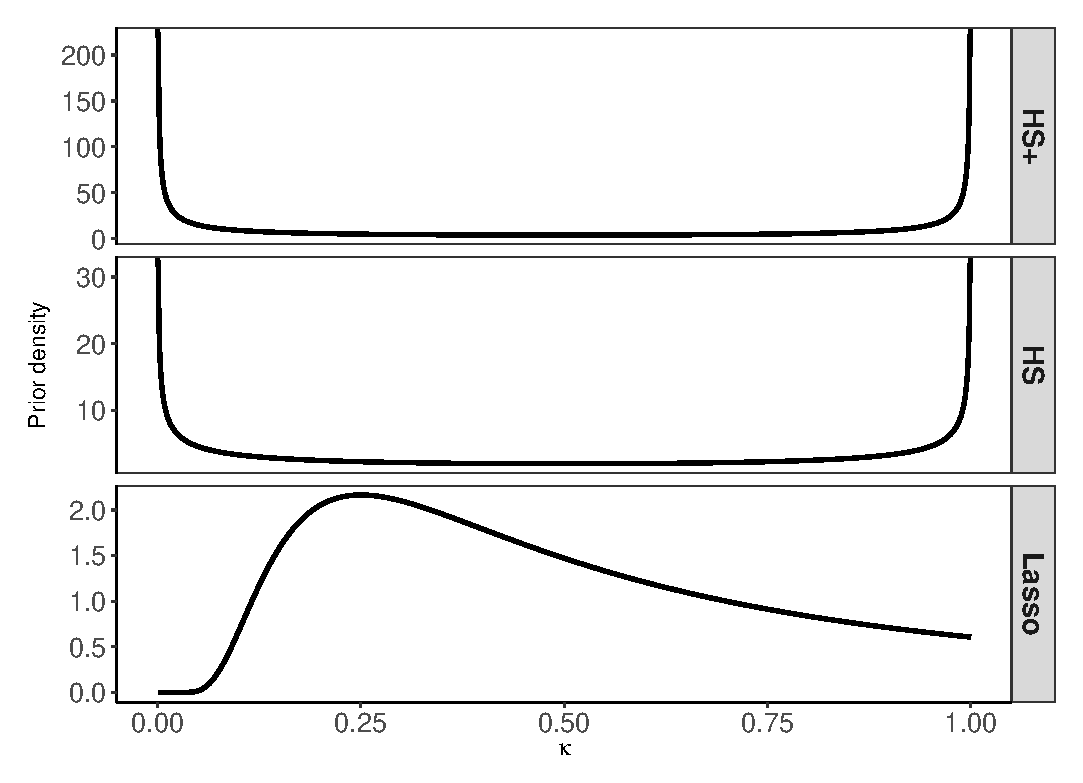
\includegraphics[width=0.48\textwidth]{prior_diff_kappa}
\caption{\footnotesize{Shrinkage profile for Horseshoe, Horseshoe+, and Laplace prior.}}
\label{fig:priorkappa}
\end{figure}
%\end{wrapfigure}
%\end{center}
%\vspace{-0.9cm}

For correlated predictors, \cite{zou2005regularization} proposed a family of
convex penalty called `elastic net', which is a hybrid between Lasso and Ridge.
The penalty term is $\sum_{j=1}^{p} \lambda p_{\alpha}(\theta_j)$, where 
\[
p_{\alpha}(\theta_j) = \half (1-\alpha)\theta_j^2 + \alpha \abs{\theta_j}, \quad j = 1, \ldots, p. 
\]
Both Lasso and Elastic net facilitate efficient Bayesian computation via a
global-local scale mixture representation \citep{bhadra2016global}. The Lasso
penalty arises as a Laplace global-local mixture \citep{andrews1974scale},
while the elastic-net regression can be recast as a global-local mixture with a
mixing density belonging to the orthant-normal family of distributions
\citep{hans2011elastic}.  The orthant-normal prior on $\theta_i$, given
hyper-parameters $\lambda_1$ and $\lambda_2$, has a density function with the
following form:
\begin{equation}
  p(\theta_i \mid \lambda_1, \lambda_2)  = 
  \begin{cases} 
   \phi(\theta_i \mid \frac{\lambda_1}{2\lambda_2}, \frac{\sigma^2}{\lambda_2}) / 2\Phi\left(-\frac{\lambda_1}{2\sigma \lambda_2^{1/2} }\right), & \quad \theta_i < 0, \\
   \phi(\theta_i \mid \frac{-\lambda_1}{2\lambda_2}, \frac{\sigma^2}{\lambda_2}) / 2\Phi\left(-\frac{\lambda_1}{2\sigma \lambda_2^{1/2} }\right), & \quad \theta_i \geq 0. \end{cases} 
  \label{eq:hans}
\end{equation}
 

\subsection{Horseshoe Penalty and Prior}
\label{sec:one-gp}

%Exponential integral function and bound $ \log (1 + 1/ \theta^2 ) $. Horseshoe \citep{carvalho2009handling, carvalho2010horseshoe, polson2010shrink, polsonscott2012} and horseshoe+ \citep{bhadra2015horseshoe+} proceed by shrinkage, so the combinatorial problem does not arise.

The horseshoe prior is a continuous ``one-group'' shrinkage rule based on what
they call the horseshoe prior for multiple testing and model selection.
Specifically, the horseshoe prior for $\theta_i$, given a global shrinkage
parameter $\tau$, is given by the hierarchical model 
\begin{align}
  (y_i \mid \theta_i) & \sim \Nor(\theta_i , \sigma^2), \;, 
  (\theta_i \mid \lambda_i, \tau) \sim 
  \Nor(0, \lambda_i^2 \tau^2) \nonumber \\ \lambda_i ^2 &
  \sim \operatorname{C}^{+}(0,1), \quad i = 1, \ldots, n. 
  \label{eq:hs}
\end{align}

As previously noted, the horseshoe prior operates under a different philosophy:
that of modeling the inclusion probability directly rather than using a
discrete mixture to model sparsity. To see this, note that the posterior mean
under the horseshoe prior can be written as a linear function of the
observation:
\begin{equation}
\E(\theta_i \mid y_i) = (1- \E(\kappa_i \mid y_i))y_i \text{ where } \kappa_i = 1/(1+\lambda_i^2 \tau^2)
\end{equation}
The name ``Horseshoe'' arises from the shape of the beta prior density of the
shrinkage weights, $\kappa_i$. A comparison with the posterior mean obtained
under the two-groups
model reveals that the shrinkage weights perform the same job as the posterior
inclusion probability $P(\theta_i \ne 0 \mid y_i)$ for recovering a sparse
signal. Since the shrinkage coefficients are not formal Bayesian posterior
quantities, we refer to them as `pseudo posterior inclusion probabilities'.
\citet{carvalho2010horseshoe} provided strong numerical evidence that this
``one-group" shrinkage rule approximately behaves like the answers from a
two-groups model under sparsity and attains super-efficiency in reconstructing
the true density. Although, the main goal of a shrinkage prior is estimation,
this interpretation of shrinkage weights as inclusion probabilities led
\citet{carvalho2010horseshoe} to propose a multiple testing rule by using a
threshold on $1-\hat{\kappa}_i$ values. \citet{datta2013asymptotic}
investigated the theoretical optimality of such a decision rule under a $0$-$1$
additive loss and showed that the horseshoe multiple testing rule attains the
Bayes oracle up to a multiplicative constant. 

There are a number of closed-form results for the posterior distribution under a
horseshoe prior. Although the prior density under the horseshoe prior doesn't
admit a closed form, we can write the horseshoe posterior mean using the
Tweedies' formula $\E(\theta \mid y) = y + \dd{\ln m(y)}{y}$, which is also
the Bayes adjustment that provides an ``optimal'' bias-variance trade-off.
For the horseshoe prior, Tweedies' formula yields
\begin{equation}
  \E(\theta_i \mid y_i, \tau) = y_i \left( 1 - \frac{2\Phi_1(\half, 1,
  \frac{5}{2},\frac{y_i^2}{2\sigma^2}, 1-\frac{1}{\tau^2})}{
  3\Phi_1(\half, 1, \frac{3}{2},\frac{y_i^2}{2\sigma^2}, 1-\frac{1}{\tau^2})} \right)
  \;,
\end{equation}
where $\Phi_1$ is the bivariate confluent hypergeometric function. This
enables one to rapidly calculate the posterior mean estimator under the
horseshoe prior via a ``plug-in'' approach with estimated values of the
hyper-parameter $\tau$. In a series of fundamental papers,
\citet{van2014horseshoe} showed that the empirical Bayes posterior mean
estimator enjoys  a ``near-minimax'' rate of estimation if the global shrinkage
parameter $\tau$ is chosen suitably. We discuss the statistical properties of
horseshoe posterior mean estimator and the induced decision rule in more
details in Section~\ref{sec:stat-prop}. 

%
The horseshoe prior is a member of a wider class of global-local scale mixtures of normals that admit following hierarchical form \citep{polson2010shrink}: 
\begin{gather*}
(\y \mid \btheta) \sim \Nor(\X \btheta, \sigma^2 \I) ;\; \theta_i \sim \Nor(0, \lambda_i^2 \tau^2) \\
\lambda_i^2 \sim \pi(\lambda_i^2) ; \; (\tau,\sigma^2) \sim  \pi(\tau^2,\sigma^2), i = 1, \ldots, n. 
\end{gather*}
These priors are collectively called ``global-local'' shrinkage priors in
\cite{polson2010shrink}, since they recover signals by a local shrinkage
parameter and adapt to sparsity by a global shrinkage parameter. Some of the
popular shrinkage priors include the Generalized Double Pareto (GDP)
\citep{armagan2013generalized}, the three-parameter Beta
\citep{armagan2011generalized}, and the more recent horseshoe+
\citep{bhadra2015horseshoe+} and the Dirichlet-Laplace
\citep{bhattacharya2014dirichlet} priors. A natural question is \textit{how do
we compare between these priors?} It is known due to several authors
\citep[e.g.]{polson2010shrink,bhadra2015default,van2015conditions} that the key
features of a global-local shrinkage prior is a peak at origin and heavy tails.
Below we list a few popular global-local shrinkage priors along with their
behaviour near origin and the tails. A detailed list of shrinkage priors
proposed in the recent past is deferred to Section~\ref{sec:app-ext}.

\begin{table}%
\centering
\begin{tabular}{| c | c |c |}
\hline
Prior & Origin Behavior & Tails \\
\hline 
Horseshoe & $-\log(\abs{\theta})$ & $\abs{\theta}^{-2}$ \\
Horseshoe+ & $-\log(\abs{\theta})$ & $\abs{\theta}^{-1}$ \\
Horseshoe-like & $-\abs{\theta}^{1-\epsilon}\log(\abs{\theta})$ & $\abs{\theta}^{1-\epsilon}$ $\epsilon \ge 0$\\
GDP & Bounded at origin & $\abs{\theta}^{-(\alpha + 1)}, \alpha \ge 0$ \\
$DL_{a}$ ($DL_{\frac{1}{n}}$) & $\abs{\theta}^{a-1}$ ($\abs{\theta}^{\frac{1}{n}-1}$) & $\exp(-b\abs{\theta})$ \\
\hline
\end{tabular}
\caption{Different Priors: Behaviour near origin and tails}
\label{tab:priors}
\end{table}

\begin{figure}[ht!]
% \centering 
  \begin{subfigure}{0.45\linewidth}
	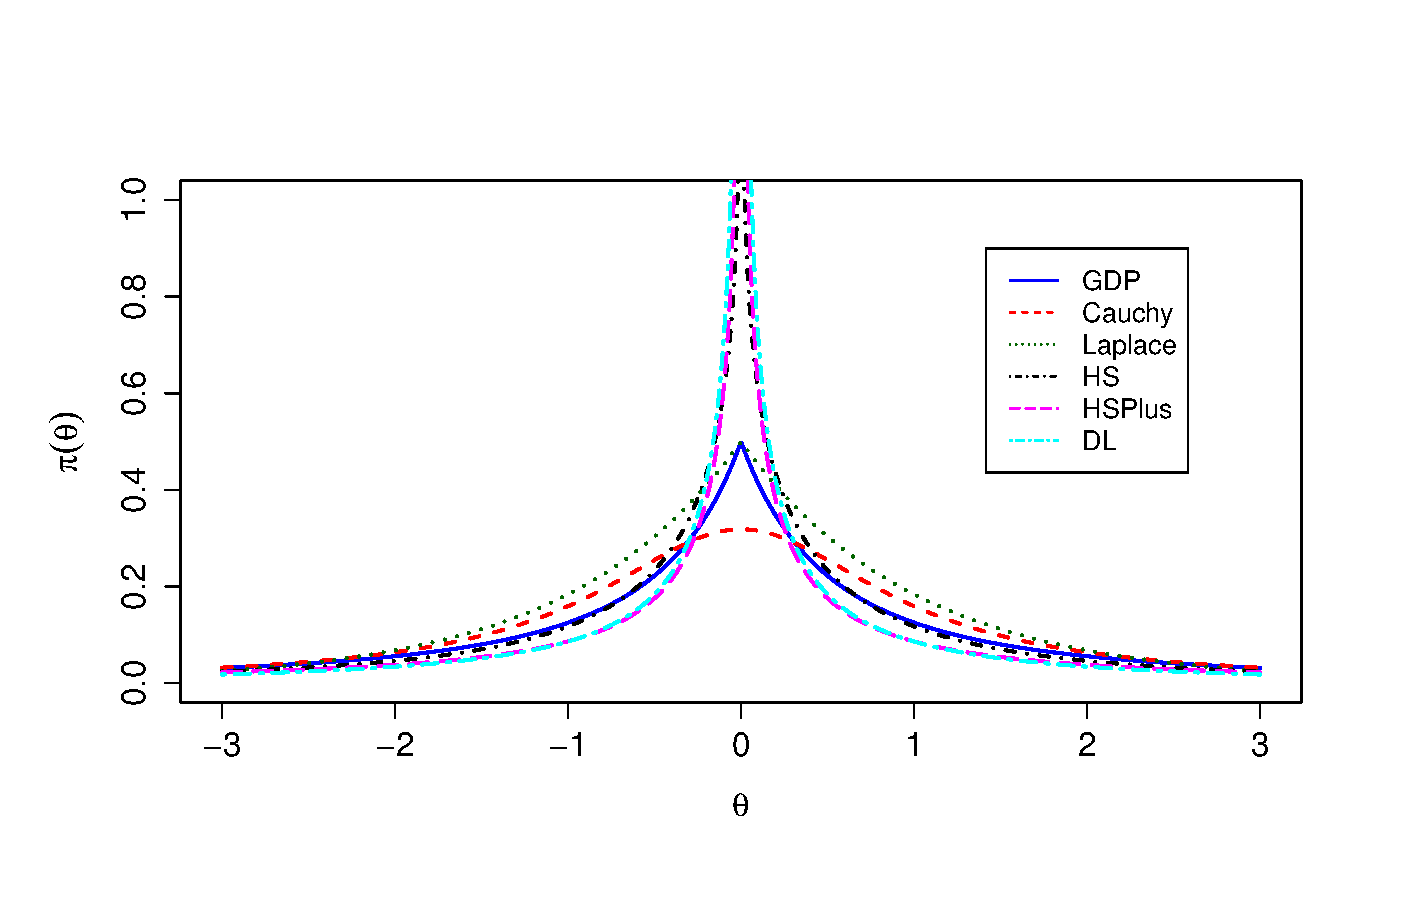
\includegraphics[height=2.5in,width=\textwidth]{densities_zero_new}%
	\caption{\footnotesize{Marginal prior densities near the origin. The legends denote the horseshoe+ (HSPlus), horseshoe (HS), Dirichlet-Laplace (DL), generalized double Pareto (GDP), Cauchy and Laplace priors.}}
	\label{fig:zero}
	\end{subfigure}
	\hspace{0.1in}
  \begin{subfigure}{0.45\linewidth}
	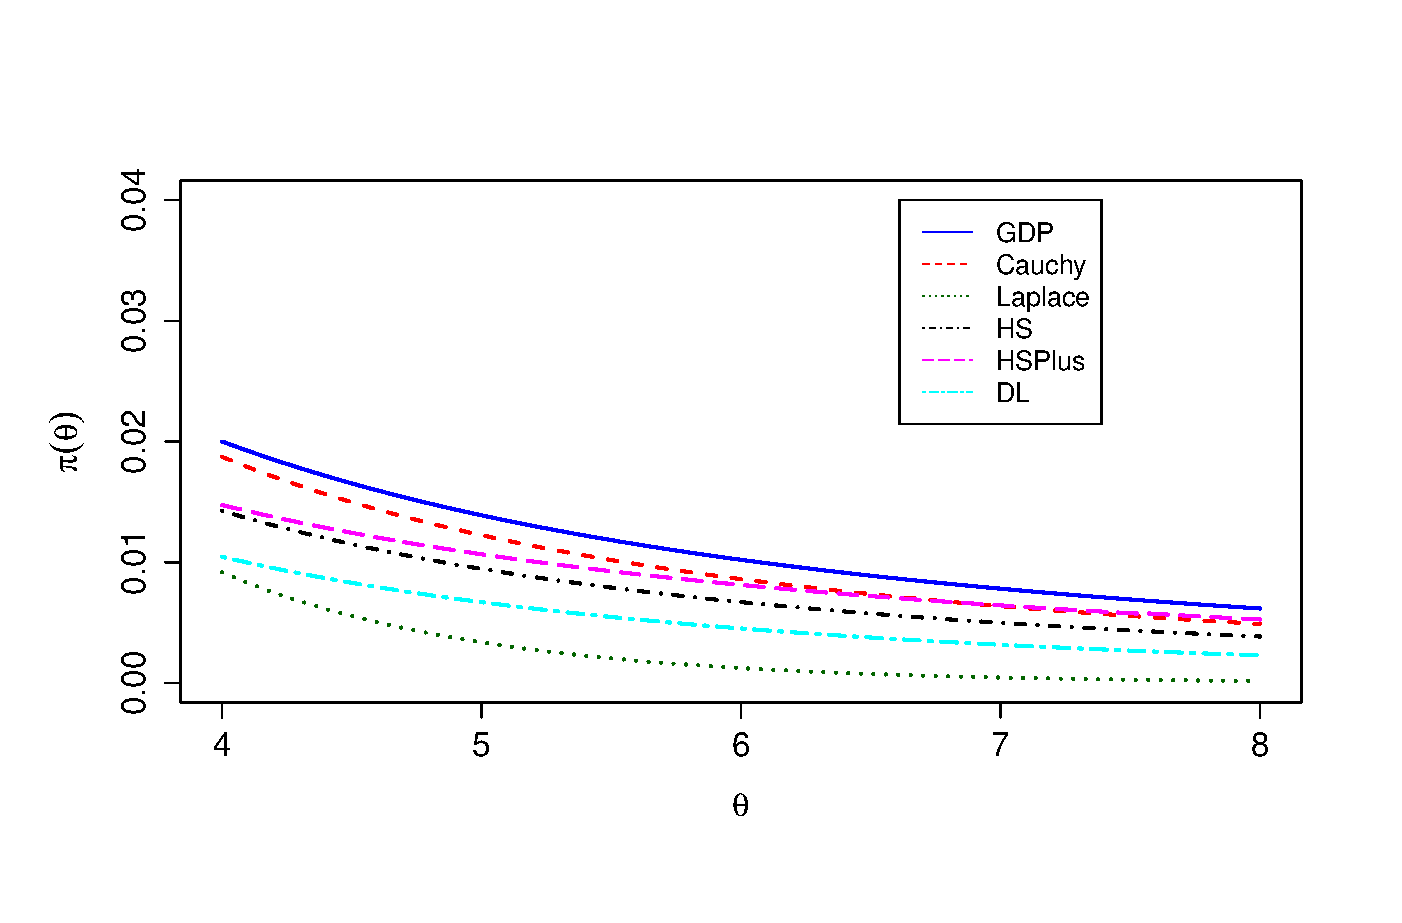
\includegraphics[height=2.5in,width=\textwidth]{densities_tails_new}
 	 \caption{\footnotesize{Marginal prior densities in the tail regions. The legends denote the horseshoe+ (HSPlus), horseshoe (HS), Dirichlet-Laplace (DL), generalized double Pareto (GDP), Cauchy and Laplace priors.}}
  \label{fig:tails}
		\end{subfigure}
\end{figure}

One way to judge a prior is by the penalty it induces in a regularisation
framework \eqref{eq:reg}. For a prior $p(\theta)$, the induced penalty is given
by $-\log p(\theta)$ as described in \eqref{eq:pen}. Although the horseshoe
prior leads to optimal performance as a shrinkage prior, the induced penalty
does not admit a closed form as the marginal prior is not analytically
tractable. This poses a hindrance in learning via Expectation-Maximization or
other similar algorithms.  The generalized double Pareto prior of
\citet{armagan2011generalized} admits a closed form solution, but it does not
have an infinite spike near zero needed for sparse recovery. Motivated by this fact,
\citet{bhadra2017horseshoe} recently proposed the ``horseshoe-like'' prior by
normalizing the tight bounds for the horseshoe prior. Thus, the horseshoe-like
prior attains a unique status within its class: it has a closed form marginal
prior for $\theta_i$, yet with a spike at origin and heavy tails and more
importantly, admits a global-local scale mixture representation. The scale
mixture decomposition supports both a traditional MCMC sampling for uncertainty
quantification in full Bayes inference and EM/MM or proximal learning when
computational efficiency is the primary concern. Since the aim of designing a
sparsity prior is achieving higher spike near zero while maintaining regularly
varying tails, a useful strategy is to split the range of the prior into
disjoint intervals: $[0,1)$ and $[1, \infty)$, and aim for higher spike in one
and heavier tail in the other. This leads to a class of `horseshoe-like' priors
with more flexibility in shape than any single shrinkage prior. We provide the
general form of horseshoe-like priors and a key
representation theorem.  See \citet{bhadra2017horseshoe} for more details. 

\begin{description}
  \item[Horseshoe-like priors] 
    \citet{bhadra2017horseshoe} have the following marginal prior density for
    $\theta_i$: 
    \begin{equation}
      \tilde p_{\tilde{HS}} (\theta_i \mid \tau^2) = \frac{1}{2 \pi{\tau}}\log
      \left ( 1 + \frac{\tau^2}{\theta_i^2} \right ), \quad  \; \theta_i  \in
      \mathbb{R},\; \tau > 0. \label{eq:hslike}
    \end{equation}
    The general family of horseshoe-like priors can be constructed as a density
    split into disjoint intervals as follows:
    \begin{align}
      p_{hs}(\theta_i \mid \tau^2)&  \propto \begin{cases}
        \frac{1}{\theta_i^{1-\epsilon}}\log \left( 1 + \frac{\tau^2}{\theta_i^2}
          \right) & \text{ if } {\abs{\theta_i} < 1} \\ \theta_i^{1-\epsilon}
          \log \left( 1 + \frac{\tau^2}{\theta_i^2} \right) & \text{ if
        }{\abs{\theta_i} \ge 1}, \\ \end{cases} \; \epsilon \ge 0,\tau > 0.
        \label{eq:split} 
    \end{align}
  \item[Normal scale mixture] 
    The horseshoe-like prior \eqref{eq:hslike} is a Gaussian scale mixture with
    a Slash normal density, which is in turn a Normal scale mixture of 
    $\operatorname{Pareto}(1/2)$ density, yielding the following representation
    theorem: 
    \begin{theorem}\label{th:hslike}
      The horseshoe-like prior in \eqref{eq:hslike} has the following global-local
      scale mixture representation:
      \begin{equation}
        \begin{gathered}
          (\theta_i \mid t_i, \tau) 
          \sim \Nor\left(0, \frac{\tau^2}{t_i^2} \right)
          ,\quad
          (t_i \mid s_i) 
          \sim \Nor\left(0, s_i \right), \; 
          \\
          s_i 
          \sim \operatorname{Pareto}\left( \frac{1}{2} \right), 
          \quad 
          t_i \in \mathbb{R}, \; \tau \ge 0.
        \end{gathered}
        \label{eq:pareto}
      \end{equation}
    \end{theorem}
\end{description}

\begin{table}[!ht]
\centering
%\def~{\hphantom{0}}
\caption{Priors for $\lambda_i$ and $\kappa_i$ for a few popular shrinkage rules}
%{\footnotesize
\begin{tabular}{ccc}
\hline
Prior for $\theta_i$ & Prior for $\lambda_i$ & Prior for $\kappa_i$ \\ 
\hline \\
%GDP & $\frac{\sqrt{2}}{(\lambda_i^2)} \int_{0}^{\infty} \exp \bigg(\sqrt{\frac{2u}{\lambda_i^2}} - u \bigg) \sqrt{u} \mathrm{d}u$  & $\frac{1}{2(1-\kappa)^2} \left[ \frac{\sqrt{\pi} \exp \left\{ \frac{\kappa}{2(1-\kappa)} \right\} Erfc \left\{ \sqrt{\frac{\kappa}{2(1-\kappa)}} \right\}  }{\sqrt{2\kappa(1-\kappa)}} - 1 \right]$ \\[20pt]
Horseshoe & $2/ \left\{ \pi \tau (1 + (\lambda_i/\tau)^2 )\right\}$  & $\frac{\tau}{\sqrt{\kappa_i (1-\kappa_i )}} \frac{1}{(1+\kappa_i (\tau^2 -1 ) )}$ \\[10pt]
Horseshoe+ & $\frac{4\log \lambda_i/\tau}{\left\{{\pi^2 \tau}(\lambda_i/\tau)^2 -1)\right\}}$ &  $\frac{\tau}{\sqrt{\kappa_i (1-\kappa_i )}}\frac{\log \left \{ ( 1 - \kappa_i ) / \kappa_i \tau^2 \right \}}{ (1-\kappa_i (\tau^2 +1 ))}$ \\[10pt]
Double Exponential & $\lambda_i \exp (-\lambda_i^2/2)$ & $\kappa_i^{-2} \exp{-\frac{1}{2\kappa_i}}$ \\
\hline 
\end{tabular}
%}
\end{table}

%\section{Bayesian Regularization : A Useful Duality }
%\subsection{Feature Extraction via Non-convex Penalty:} For the sparse normal means model where $\#(\theta_i \ne 0)\le p_n$ and $p_n = o(n)$ as $n \to \infty$, non-convex regularization problems arise from a need to correctly identify the zero components in $\theta$, also known as subset selection. The  $\ell_0$ penalty, defined as $||\theta||_0 =\sum_{i=1}^{n} 1(|\theta_i|>0)$, is ideal for this task, and the more commonly used lasso or convex $\ell_1$ penalty, $||\theta||_1 = \sum_{i=1}^{n} |\theta_i|$, tends to select a denser model \citep{mazumder2012}. Unfortunately, naively using the $\ell_0$ penalty requires a combinatorial evaluation of all $2^n$ models, which is NP-hard \citep{natarajan95}. Penalties of the form $\ell_\gamma$ for $\gamma \ge 1$ give rise to convex problems and efficient solvers are available. It remains a challenge to fit models with $\ell_\gamma$ penalties for $\gamma\in (0,1)$. While this does not necessarily a present combinatorial problem, the regularization problem is non-convex. Thus, the general purpose tools for convex optimization do not apply, nor is a unique solution guaranteed \citep[see, e.g.,][Chapter 1]{boyd2004convex}. 
%Non-convex penalties include the smoothly clipped absolute deviation or SCAD \citep{fan2001variable} and the minimax concave penalty or MCP \citep{zhang2010nearly}. Recent computational advances in fitting models with non-convex penalties include \citet{breheny2011coordinate} and \citet{mazumder2012}. Both works use coordinate descent approaches to fit SCAD and MCP and provide conditions for convergence.  Alternatively, an overview of proximal algorithms for non-convex optimization can be found in \citet{polson2015proximal}. Recent works have also demonstrated the equivalence between fitting a model with MCP penalty and evaluating the posterior mode in a Bayesian hierarchical model under a suitable prior \citep{strawderman2013hierarchical, schifano2010majorization}. Following along these lines, we show that evaluating the posterior mode under a suitable approximation to the horseshoe prior of \citet{carvalho2009handling, carvalho2010horseshoe} solves a non-convex optimization problem with desirable theoretical properties and derive a fast computational algorithm. %Using a latent variable representation in our probabilistic framework, we develop an expectation-maximization (E-M) algorithm \citep{dempster1977} that quickly reaches a local optimum, usually in a fraction of time required by the non-convex solvers.
%\cite{bhadra2017horseshoe} provides results on feature selection properties of horseshoe-like penalties. 

\section{Statistical Risk Properties}\label{sec:stat-prop}

\paragraph{History of Shrinkage Estimation: Inadmissibility of MLE } The story
of shrinkage estimation goes back to the proof in
\citet{stein_inadmissibility_1956} that the maximum likelihood estimators for
normal data are inadmissible beyond $\mathbb{R}^2$. The James-Stein (JS) estimator
is $\hat{\theta}^{JS} = (1 - \nicefrac{(m-2)}{\vectornorm{\y}^2})\y$ with
posterior mean $\hat{\theta}_{\mathrm{Bayes}} = (\nicefrac{\tau^2}{\tau^2+1})
\y$, which corresponds to the Bayes risk of $m(\nicefrac{\tau^2}{\tau^2+1})$.
%Without any prior guess about $\tau^2$, one could use an Empirical Bayes
estimate and the resulting JS estimator is $\hat{\theta}^{JS} = (1 -
\nicefrac{m-2}{\vectornorm{\Y}^2})Y$. 
\citet{james_estimation_1961} proved that this estimator dominates the MLE in
terms of the expected total squared error for every choice of $\btheta$, i.e.
it outperforms the MLE no matter what the true $\btheta$ is. To motivate the
need for developing new prior distributions, consider the classic James--Stein
``global'' shrinkage rule, $\estJs(\y)$. The JS estimator uniformly dominates the
traditional sample mean estimator, $\hat{\theta}$. For all values of the true
parameter $\theta$ and for $n>2$, we have the classical mean squared error
(MSE) risk bound:
\[ 
  R(\estJs, \btheta) \defeq \E_{y \mid \btheta} {\Vert \estJs(\y) - \btheta
  \Vert}^2 < n = \E_{\y \mid \btheta} {\Vert \y - \btheta \Vert}^2, \quad
  \forall \btheta \in \mathbb{R}^n, \; n \ge 3.  
\]

For sparse signal problem the standard James-Stein shrinkage rule, $
\hat{\theta}_{JS} $, performs poorly. This is best seen in the sparse setting
for a $r$-spike parameter value $ \theta_r$ with $r$ coordinates at $
\sqrt{n/r} $ which has $ \Vert \theta \Vert^2 =n $.
\citet{johnstone2004needles} show that $ E \Vert \hat{\theta}^{JS} - \theta
\Vert \leq n $ with risk $2$ at the origin. Moreover, we can bound
\[
  \frac{n \Vert \theta \Vert^2}{ n + \Vert \theta \Vert^2} \leq R \left (
  \hat{\theta}^{JS} , \theta_r \right ) \leq 2 + \frac{n \Vert \theta \Vert^2}{ n
  + \Vert \theta \Vert^2},
\]
and so $\estJs(\y)$ for the $r$-spike parameter value has risk at least $ R
\left( \hat{\theta}^{JS} , \theta_r \right) \geq (n/2)$. This is nowhere near
optimal. As \citet{donoho1994ideal} showed, simpler rules such as the
hard-thresholding and soft-thresholding estimates given by
$\hat{\theta}^{H}(y,\lambda) = y I\{\abs{y} \ge \lambda \}$ and
$\hat{\theta}^{S}(y,\lambda) = sgn(y) (\abs{y} - \lambda)_{+}$ satisfy an
Oracle inequality. In particular, when the thresholding sequence is close to
$\sqrt{2\log n}$ (`universal threshold'), these estimators attain the
``oracular risk'' up to a factor of $2\log(n)$. Intuitively, this is not
surprising as the high-dimensional normal prior places most of its mass on
circular regions -- and does not support sparse, spiky vectors. 

\paragraph{Near minimax $\ell_2$ risk}

The asymptotically minimax risk rate in $\ell_2$ for nearly black objects is
given by \citet{donoho1992maximum} to be $p_n \log \left ( n / p_n \right )$.
Here $a_n \asymp b_n$ means $\lim_{n\to\infty} a_n/b_n=1$. Specifically, for
any estimator $\delta(Y)$, we have a lower bound: 
\begin{equation}
  \sup_{\theta_0 \in \ell_0[p_n]} \E_{\theta_0} \norm{\delta(Y) - \theta_0}^2
  \ge 2 \sigma^2 p_n \log(n/p_n)(1+o(1))
\end{equation}
The minimax rate, which is a frequentist criteria for evaluating the
convergence of point estimators to the underlying true parameter, is a
validation criteria for posterior contraction as well. This result, due to
\citet{ghosal2000}, showed that the minimax rate is the fastest that the
posterior distribution can contract. 

Horseshoe estimators enjoy ``near-minimax'' rates in both an empirical Bayes and
full Bayes approach, provided that the hyper-parameters or the priors are
suitably chosen--as proved in a series of papers
\citep{van2014horseshoe,van2015conditions,van2016many,van2017adaptive}.
Specifically, the horseshoe estimator achieves
\begin{equation}
  \sup_{ \theta \in l_0[p_n] } \; \mathbb{E}_{ y | \theta } \norm{ \estHs (y) -
  \theta }^2 \asymp p_n \log \left ( n / p_n \right ), 
  \label{eq:minimax}
\end{equation}
\citet{van2014horseshoe} showed that the near-minimax rate can be achieved by
setting the global shrinkage parameter $\tau = (p_n/n) \log(n/p_n)$. In
practice, $\tau$ is unknown and must either be estimated from the data or
handled via a fully Bayesian approach by putting a suitable prior on $\tau$.
\cite{van2017adaptive} show that the theoretical optimality properties for the
popular horseshoe prior holds true if the global shrinkage parameter $\tau$ is
learned via the maximum marginal likelihood estimator (MMLE) or a full Bayes
approach. For the full Bayes estimator, these conditions are easily seen to
satisfied by a half-Cauchy prior truncated to the interval $[1/n,1]$, which
also does well in numerical experiments, both in `sparse' and `less-sparse'
situations. Independently, \citet{van2015conditions} and
\citet{ghosh2016asymptotic} showed that these optimality properties are not
unique features of the horseshoe prior and they hold for a general class of
global-local shrinkage priors. While the results of \cite{van2015conditions}
apply to a wider class of priors, including the horseshoe+ prior
\citep{bhadra2015horseshoe+} and spike-and-slab Lasso
\citep{rovckova2016spike}.  We note that \citet{ghosh2016asymptotic} attain
sharper mean-squared error bounds. 

\paragraph{Lasso}

A natural question is how does the Lasso fare in these aspects? While the MAP estimator under the Bayesian formulation of Lasso (i.e. i.i.d. Laplace prior on $\theta_i$'s) enjoys all the desirable properties of the frequentist Lasso, it is known to be sub-optimal for recovery of the underlying $\btheta_0$ \citep{castillo2012needles}. In fact, \cite{castillo2012needles} show that unlike the mode, the full posterior distribution under the Laplace prior does not contract at the optimal rate, making it `useless for \textit{uncertainty quantification}'. 

%\begin{enumerate}
%\item  \citet{van2014horseshoe} showed it for horseshoe.
%\item  \citet{van2015conditions} showed it for horseshoe+ and several other ``global-local'' models.
%\item \citet{ghosh14} is similar to  \citet{van2015conditions}.
%\item \citet{van2016many} is a new paper that we need to read and possibly cite. 
%\end{enumerate}

\paragraph{Asymptotic Bayes Optimality under Sparsity}

One of main reasons behind the widespread popularity of Lasso is the in-built
mechanism for performing simultaneous shrinkage and selection. The frequentist
Lasso or the equivalent MAP estimator under i.i.d.  The double-exponential
prior induces automatic sparsity and can be easily adjusted to achieve model
selection consistency. The horseshoe estimator, on the other hand, is a
shrinkage rule that induces a selection rule through thresholding the pseudo
posterior inclusion probabilities. Thus, we can compare their relative
performance for multiple testing under the two-groups model and a $0$-$1$
additive loss framework. It turns out that for large scale testing problems the
horseshoe prior attains the ``oracle'' property while double-exponential tails prove
to be insufficiently heavy, leading to a higher misclassification rate compared
to the Horseshoe prior. The main reasons behind the horseshoe prior's
optimality are the posterior density of shrinkage weights that can pushes most
of the density to $0$ and $1$ and the adaptability of the global shrinkage
parameter $\tau$. 

The posterior distribution under the horseshoe prior leads to a natural model
selection strategy under the two-groups model. \citet{carvalho2010horseshoe}
argued that the shrinkage coefficient $1-\hat{\kappa}_i$ can be viewed as
a pseudo-inclusion probability $P(\theta_i \ne 0 \mid y_i)$ and induces a
multiple testing rule.
\begin{equation}
  \text{Reject the $i^{th}$ null hypothesis } H_{0i} : \theta_i = 0 \text{ if }
  1-\hat{\kappa}_i > \half \;. 
  \label{eq:hsrule}
\end{equation}
Under the two-groups model \eqref{twogroups}, and a $0$-$1$ loss, the Bayes risk is 
\[
R = \sum_{i=1}^{n} \{ (1- \pi) t_{1i} + \pi t_{2i} \}
\]

If we know the true values of the sparsity and the parameters of the non-null
distribution, we can derive a decision rule that is impossible to beat in
practice, this is called the Bayes Oracle for multiple testing
\citep{bogdan2011asymptotic}. The ``oracular risk'' serves as the lower bound
for any multiple testing rule under the two-groups model and thus provides an
asymptotic optimality criteria when the number of tests go to infinity. The
asymptotic framework of \citet{bogdan2011asymptotic} is 
\begin{equation}
p_n \to 0, \; u_n = \psi_n^2 \to \infty, \; \text{and} \; \log(v_n)/u_n \to C \in (0,\infty) \label{eq:asymp}
\end{equation}
where $v_n = \psi_n^2 (\frac{1-p_n}{p_n})^2$. The Bayes risk for the Bayes oracle under the above framework \eqref{eq:asymp} is given by:
\[
R_{\text{Oracle}} = n \pi (2 \Phi(\sqrt{C}) - 1)(1+o(1))
\]
A multiple testing rule is called ABOS (asymptotic Bayes optimal under
sparsity) if it attains the oracular risk as $n \to \infty$.
\citet{bogdan2011asymptotic} provided conditions for a few popular testing
rules, e.g. Benjamini--Hochberg FDR controlling rule to be ABOS.
\citet{datta2013asymptotic} first showed that the decision rule
\eqref{eq:hsrule} is also ABOS up to a multiplicative constant if $\tau$ is
chosen suitably to reflect the sparsity, namely $\tau = O(\pi)$.
The proof in \citet{datta2013asymptotic} hinges on the concentration of the posterior
distribution near $0$ and $1$, depending on the trade-off between signal
strength and sparsity.  In numerical experiments,
\citet{datta2013asymptotic} also confirmed that the horseshoe prior
induced rule outperforms the shrinkage rule induced by the double-exponential
prior under various levels of sparsity. 
Although $\tau$ is treated as a tuning parameter that mimics $\pi$ in the
theoretical treatment, in practice, $\pi$ is an unknown parameter. Several
authors \cite{datta2013asymptotic, ghosh2016asymptotic,
ghosh2016testing,van2016many} have shown that usual estimates of $\tau$ adapts
to sparsity, a condition that also guarantees near-minimaxity in estimation.
\citet{ghosh2016testing} extended the ABOS property to a wider class of
global-local shrinkage priors, with conditions on the slowly varying tails of
the local shrinkage prior. They have also shown that the testing rule under a
horseshoe-type prior is \textit{exactly} ABOS, when $\lim_{n \to \infty} \tau/p
\in (0, \infty)$. 


%\subsection{Prediction using global-local priors}
%\begin{enumerate}
%\item \citet{ carvalho2010horseshoe}: K-L superefficiency for predictive density for horseshoe.
%\end{enumerate}

\section{Hyper-parameter Tuning}

\paragraph{Optimization and Cross-validation}

Careful handling of the global shrinkage parameter $\tau$ is critical for
success of the horseshoe estimator in a sparse regime as it captures the level
of sparsity in the data \citep{carvalho2010horseshoe, datta2013asymptotic,
van2015conditions, van2016many}. However, in nearly black situation a naive
estimate of $\tau$ could collapse to zero, and care must be taken to prevent
possible degeneracy in inference. There are two main approaches regarding
choice of $\tau$: first, a fully Bayesian approach that specifies a hyper-prior
on $\tau$ and second, an empirical Bayesian approach that estimates $\tau$ from
the data using a simple thresholding or maximum marginal likelihood approach
(MMLE). In a recent paper, \citet{van2017adaptive} have investigated the
empirical Bayes and full Bayes approach for $\tau$, and have shown that the
full Bayes and the MMLE estimator achieve the near minimax rate, namely $p_n
\log(n)$, under similar conditions. For the full Bayes estimator, these
conditions are easily seen to satisfied by a half-Cauchy prior truncated to the
interval $[1/n,1]$, which also does well in numerical experiments, both in
`sparse' and `less-sparse' situations. 

The MMLE estimator of \citet{van2017adaptive} outperforms the simple
thresholding estimator given by
\[
  \hat{\tau}_s(c_1, c_2) = \max \left \{ \frac{\sum_{i=1}^{n} \1 \{ \abs{y_i} \ge
  \sqrt{c_1 \log(n) \}}}{c_2 n}, \frac{1}{n} \right\}
  \;.
\]
Rather, the MMLE estimator can detect smaller non-zero signals, even those below the threshold $\sqrt{2 \log(n)}$, such as $\theta_i = 1$ when $n = 100$. 
The success of the MMLE estimator, both theoretically and numerically,
challenges the notion that for the horseshoe prior an empirical Bayes parameter
estimate of $\tau$ cannot replace a full Bayes estimate of $\tau$. In reality,
one must take care to prevent the estimator from getting too close to zero. 

A third approach could be treating $\tau$ as a tuning parameter and using a
$k$-fold cross-validation to select $\tau$.  As in the full Bayes and empirical
Bayes approach, the cross-validated choice of $\hat{\tau}$ can also converge to
zero and care should be taken to avoid zero in such situations. Yet another
approach for handling $\tau$ was proposed by \citet{piironen2016hyperprior},
who have investigated the choice of $\tau$ for a linear regression model and
have suggested choosing a prior for $\tau$ by studying the prior for
$m_{\text{eff}} = \sum_{i=1}^{n} (1-\kappa_i)$, the effective number of
non-zero parameters. 

%Path (computational speed), Sensitivity Analysis. Cross-validation approach (has caveats), marginal MLE, $\argmax_{\tau} p(y \mid \tau)$. Plug-in estimators can be inadmissible, SURE: procedure. 

\paragraph{Marginal Likelihood: } We now take a closer look at how $\tau$
affects the marginal likelihood under the horseshoe prior and the maximum
marginal likelihood approach of \cite{van2017adaptive}. 
We can write the marginal likelihood under the horseshoe prior in \eqref{eq:hs}
after marginalising out $\theta_i$ from the model as:
\begin{equation}
  m(y \mid \tau) = \prod_{i=1}^{n} (1+\lambda_i^2 \tau^2)^{-\half} \exp \left
  \{ - \frac{y_i^2}{2(1+\lambda_i^2 \tau^2)} \right \}  (1+\lambda_i^2)^{-1} d
  \lambda_i 
\end{equation}
\citet{tiao1965bayesian} observe that the marginal likelihood is positive at 
$\tau = 0$, hence the impropriety of the prior of $\tau^{-2}$ at the origin
translates to the posterior. As a result, a maximum likelihood estimator of
$\tau$ has a potential danger of collapsing to zero in very sparse problems
\citep{polson2010shrink, datta2013asymptotic}. In \cite{van2017adaptive}, 
both the empirical Bayes MMLE and the full Bayes solution are
restricted in the interval $[1/n,1]$ to pre-empt this behaviour. To get the
MMLE of $\tau$ using the approach of \cite{van2017adaptive}, we first calculate the
marginal prior of $\theta_i$ after integrating out $\lambda_i^2$ in 
Equation~\eqref{eq:hs}:
\begin{equation}
  p_{\tau}(\theta_i) = \int_{0}^{\infty} \frac{1}{\sqrt{2 \pi}} \exp \left\{ -
  \frac{\theta_i^2}{2\lambda^2 \tau^2} \right\} \frac{1}{\lambda \tau}
  \frac{2}{\pi(1+\lambda^2)} d\lambda
  \;.
\end{equation}
The MMLE is then obtained as the maximizer of the marginal likelihood
restricted to the interval $[1/n,1]$: 
\begin{equation}
  \hat{\tau}_M = \argmax_{\tau \in [1/n,1]} \prod_{i=1}^{n}
  \int_{-\infty}^{\infty} \frac{1}{\sqrt{2 \pi}} \exp \left\{ - \frac{(y_i
  -\theta_i)^2}{2} \right\} p_{\tau}(\theta_i) d\theta_i
  \;.
\end{equation}
The lower bound of the maximization interval prevents against a degenerate
solution of $\tau$ in sparse case. 

%The marginal likelihood is decreasing at zero when the $S_i$'s are small
%enough to make the exponential term nearly constant \citep{tiao1965bayesian}. This is precisely the sparse coefficient case.
%
%A number of default choices have been proposed to overcome this issues.
%\citet{morris2011estimating} propose a flat prior $ p( \tau ) \equiv 1 $. The tails of the likelihood are sufficient so as to lead to a proper posterior. This is also related to Stein's harmonic prior $ || \theta ||^{-(k-2)} $ for $ k \geq 3 $.  

%Methods for choosing $\tau$ will involve minimizing some criteria: %such as AIC \citep{akaike74}, BIC \citep{schwarz1978}, DIC \citep{spiegelhalter2002bayesian}, SURE \citep{stein81}, $C_p$ \citep{mallows73}. \citet{castillo2015bayesian} compared full Bayes MCMC with empirical Bayes and plug-in approaches.

\section{Computation and Simulation}\label{sec:horse-comp}

Over the last few years, several different implementation of the horseshoe prior for normal means and regression model has been proposed. The MCMC based implementations usually proceed via block-updating $\btheta$, $\blambda$ and $\tau$ using either a Gibbs or parameter expansion or slice sampling strategy. The first \textsc{R} package to offer horseshoe prior for regression along with Lasso, Bayesian Lasso and Ridge was the \texttt{monomvn} package by \citet{gramacy2010shrinkage}. In an unpublished technical report, \citet{scott_parameter_2010} proposed a parameter expansion strategy for the horseshoe prior and studied its effect on the autocorrelation of $\tau$. Furthermore, \citet{scott_parameter_2010} pointed out that the solution to this lies in marginalizing over the local shrinkage parameter $\lambda_j$'s. On a somewhat similar route, \citet{makalic2016high} uses a inverse-gamma scale mixture identity to construct a Gibbs sampling scheme for horseshoe and horseshoe+ prior for linear regression as well as logistic and negative binomial regression. The \texttt{horseshoe} package implements the MMLE and truncated prior approaches for handling $\tau$ proposed in \citet{van2017adaptive}. \citet{hahn_elliptical_2016} proposed an elliptical slice sampler and argues that it wins over Gibbs strategies for higher dimensional problems both in per-sample speed and quality of samples (i.e. effective sample size). The state-of-the-art implementation for horseshoe prior in linear regression is \citet{bhattacharya_fast_2015} who used a Gaussian sampling alternative to the na\''ive Cholesky decomposition to reduce the computational burden from $O(p^3)$ to $O(n^p)$. A very recent paper by \citet{james2017scalable} claims to improve this even further by implementing a block update strategy but using a random walk Metropolis--Hastings algorithm on $\log(1/\tau^2)$ for block-updating $\tau \mid \lambda$. We provide a list of all the implementations known to us on Table \ref{tab:hs-imp}.

% Table generated by Excel2LaTeX from sheet 'Sheet1'
\begin{table}[htbp]
  \centering
  \caption{Implementations of Horseshoe and Other Shrinkage Priors}
  \footnotesize{
    \begin{tabular}{|c|c|}
    \hline
    Implementation (Package/URL) & Authors \bigstrut\\
    \hline
    \textsc{R} package: \href{https://cran.r-project.org/web/packages/monomvn/index.html}{\texttt{monomvn}} & \citet{gramacy2010shrinkage} \bigstrut[t]\\
     \textsc{R} code in paper & \citet{scott_parameter_2010} \\
    \textsc{R} package: \href{https://cran.r-project.org/web/packages/horseshoe/index.html}{\texttt{horseshoe}} & \citet{pas_horseshoe:_2016} \\
    \textsc{R} package: \href{https://cran.r-project.org/web/packages/fastHorseshoe/index.html}{\texttt{fastHorseshoe}} & \citet{hahn_elliptical_2016} \\
    \href{https://github.com/antik015/Fast-Sampling-of-Gaussian-Posteriors}{\textsc{Matlab} code} & \citet{bhattacharya_fast_2015} \\
    GPU accelerated Gibbs sampling & \citet{terenin_gpu-accelerated_2016} \\
    \href{https://cran.r-project.org/web/packages/bayesreg/index.html}{\texttt{bayesreg}} + \textsc{Matlab} code in paper & \citet{makalic2016high} \\
     \href{https://github.com/jamesjohndrow/horseshoe_jo}{\textsc{Matlab} code} & \citet{james2017scalable} \bigstrut[b]\\ 
    \hline
    \end{tabular}%
    }
  \label{tab:hs-imp}%
\end{table}%


%\begin{enumerate}
%\item Mention R package. 
%\item Compare with various methods.
%\end{enumerate}


\section{Applications and Extensions}\label{sec:app-ext}

%Literature review of applications and extensions and recent development. List papers. 
%Fused and group lasso. Extension to logistic (Polya-Gamma for logistic : MCMC still convex). 

\paragraph{Applications and Extensions of Lasso:} Since the inception of Lasso
as a regularisation method for linear regression in 1996, a great deal of
extensions and applications have been proposed in the literature. The combined
effect of convex penalty and sparsity of the final solution lead to huge
computational gains by using powerful convex optimization methods on problems
of massive dimensions. The coordinate descent approach
\citep{friedman2007pathwise,friedman2010regularization} is one particularly
promising approach, that works by applying soft-threshold to the least-squares
solution obtained on partial residuals, one at a time. The coordinate descent
approach is flexible and easy and can be proved to converge to the solution as
long as the log-likelihood and penalty are convex \citep{tseng2001convergence},
paving the way for wide applicability of $\ell_1$ penalty in generalized linear
models (GLM). The popular R package \texttt{glmnet} provides a nice and easy
interface for applying Lasso and elastic-net penalty for a general sparse GLM.
Although a comprehensive list of regularization methods that extend the idea of
Lasso and even move beyond the convex penalty is beyond the scope of this
article, we give a list of popular regularization methods in 
Table~\ref{tab:lasso:ext}, which is adapted from \citet{tibshirani2014praise}.

% Table generated by Excel2LaTeX from sheet 'Sheet1'
\begin{table}[ht!]
  \centering
  \caption{A few regularization methods}
  \footnotesize{
    \begin{tabular}{|c|c|}
    \hline
    Method  & Authors  \bigstrut\\
    \hline
    Adaptive Lasso & \citet{zou2006adaptive} \bigstrut[t]\\
    Compressive sensing  & \citet{donoho2006compressed,candes2008restricted} \\
    Dantzig selector  & \citet{candes2007dantzig} \\
    Elastic net & \citet{zou2005regularization} \\
    Fused Lasso & \citet{tibshirani2005sparsity} \\
    Generalized Lasso & \citet{tibshirani2011solution} \\
    Graphical Lasso & \citet{friedman2008sparse} \\
    Grouped Lasso & \citet{yuan2006model} \\
    Hierarchical interaction models & \citet{bien2013lasso} \\
    Matrix completion & \citet{candes2010power,mazumder2010spectral} \\
    Multivariate methods & \citet{jolliffe2003modified,witten2009penalized} \\
    Near-isotonic regression & \citet{tibshirani2011nearly} \\
    Square Root Lasso  & \citet{belloni2011square} \\
    Scaled Lasso & \citet{sun2012scaled} \\
    Minimum concave penalty & \citet{zhang2010nearly} \\
    SparseNet & \citet{mazumder2012} \bigstrut[b]\\
    \hline
    \end{tabular}%
    }
  \label{tab:lasso:ext}%
\end{table}%

\paragraph{Applications and Extensions of Horseshoe:}

As discussed in Section~\ref{sec:one-gp}, the Horseshoe prior belongs to a wider class of global-local shrinkage priors \citep{polson2010shrink} that are characterized by a local shrinkage parameter for recovering large signals and a global shrinkage parameter for adapting to overall sparsity. The class of global-local priors, although differing in their specific goals and design, exhibit some common features: heavy tails for tail-robustness and appreciable mass near zero for sparsity, leading to shared optimality properties. Several authors including \citet{van2015conditions, ghosh2016asymptotic, ghosh2016testing} have provided conditions for optimality of one-group continuous priors for estimation of sparse normal means and multiple testing. Table \ref{tab:one-gps} provides a sampling of a few continuous shrinkage priors popular in the literature. 

Although the original horseshoe prior was developed for signal recovery with
sparse Gaussian means, the idea of directly modeling the posterior inclusion
probability and use of normal-scale mixture to facilitate sparsity is a
flexible idea and can be easily generalized to a wider class of problems.
\citet{bhadra2015default} show that the horseshoe prior is a good candidate as
a default prior for low-dimensional, possibly non-linear functionals of
high-dimensional parameter and can resolve long-standing marginalization
paradoxes for such problems. \citet{bhadra2016prediction} show how to use
global-local priors for prediction and provide theoretical and numerical
evidence that it performs better than a variety of competitors including Lasso,
Ridge, PCR and sparse PLS. 

Moving beyond Gaussianity, \citet{datta2016bayesian} re-discovered the
Gauss-hypergeometric prior for flexible shrinkage needed for quasi-sparse count
data, with a tighter control on false discoveries.
\citet{piironen2016hyperprior} used a Gaussian approximation using a
second-order Taylor expansion for the log-likelihood to apply the horseshoe
prior for the generalized linear model. \citet{wang2013class} proposed a
shrinkage prior based on a scale mixture of uniform for covariance matrix
estimation. \citet{peltola2014hierarchical} applies the horseshoe prior for
Bayesian linear survival regression for selecting covariates with highest
predictive values. A sample of the many applications of horseshoe prior is
given in Table \ref{tab:hs-apps}. Given the explosive growth of the methods in
this area, we conjecture that the horseshoe prior would be regarded as a key
tool sparse signal recovery and as a default prior for objective Bayesian
inference for many important problems. 

% Table generated by Excel2LaTeX from sheet 'Sheet1'
\begin{table}[htbp]
  \centering
  \caption{A catalogue of global-local shrinkage priors}
  \footnotesize{
    \begin{tabular}{|c|c|}
    \hline
    Global-local shrinkage prior  & Authors  \bigstrut\\
    \hline
    Normal Exponential Gamma & \citet{griffin2005alternative} \bigstrut[t]\\
    Horseshoe & \citet{carvalho2010horseshoe, carvalho2009handling} \\
    Hypergeometric Inverted Beta & \citet{polson2010large} \\
    Generalized Double Pareto & \citet{armagan2011generalized} \\
    Generalized Beta  & \citet{armagan2013generalized} \\
    Dirichlet-Laplace & \citet{bhattacharya2014dirichlet} \\
    Horseshoe+  & \citet{bhadra2015horseshoe+} \\
    Horseshoe-like & \citet{bhadra2017horseshoe} \\
    Spike-and-Slab Lasso & \citet{rovckova2016spike} \\
    R2-D2 & \citet{zhang2016high} \bigstrut[b]\\
    \hline
    \end{tabular}%
    }
  \label{tab:one-gps}%
\end{table}%

% Table generated by Excel2LaTeX from sheet 'Sheet1'
\begin{table}[htbp]
  \centering
  \caption{Applications of the horseshoe prior}
  \footnotesize{
    \begin{tabular}{|p{3in}|p{1.5in}|}
    \hline
    Application  & Authors \bigstrut\\
    \hline
    \textit{Fadeout} method for mean-field variational inference under non-centered parameterizations and stochastic variational inference for undirected graphical model.  & \citet{ingraham_bayesian_2016} \bigstrut[t]\\
    \hline
    Linear regression for Causal inference and Instrumental variable models  & \citet{hahn_shrinkage_2014, hahn_elliptical_2016} \\
    \hline
    Multiclass prediction using DOLDA (Diagonally orthant Latent Dirichlet Allocation)  & \citet{magnusson_dolda_2016} \\
    \hline
    Mendelian Randomization to detect causal effects of interest & \citet{berzuini_mendelian_2016} \\
    \hline 
    Locally adaptive nonparametric curve fitting with shrinkage prior Markov random field (SPMRF) & \citet{faulkner_bayesian_2015} \\
    \hline
    Quasi-Sparse Count Data & \citet{datta2016bayesian} \\
    \hline
    Variable Selection under the projection predictive framework  & \citet{piironen_projection_2015} \bigstrut[b]\\
    \hline
    \end{tabular}%
    }
  \label{tab:hs-apps}%
\end{table}%


%\begin{enumerate}
%\item \citet{bhadra2015default} use global-local priors in default Bayes Efron problems.
%\item \citet{bhadra2016prediction} show how to use global-local priors for prediction. Performs better than a variety of competitors including lasso, ridge, PCR and sparse PLS.
%\item \citet{datta2015inference} use global-local priors to model the rate parameter for Poisson count data.
%\end{enumerate}


\section{Discussion}

Lasso and Horseshoe prior regularization--and the general class of global-local
shrinkage priors--are widely used for sparse signal recovery in high
dimensional data. The horseshoe prior offers better computational efficiency
than the Bayesian two-group priors, while still mimicking the inference and it
outperforms the estimator based on Laplace prior, the Bayesian dual of Lasso.
The intuitive reason for better performance by the horseshoe prior is its heavy
tails and probability spike at zero, which makes it adaptive to sparsity and
robust to large signals.  A number of MCMC sampling algorithms have been proposed
for both the Lasso and the horseshoe prior, based on variants of coordinate
descent and MCMC respectively.  We have outlined the distinct algorithmic
implementations in \ref{sec:horse-comp} and Table~\ref{tab:hs-imp}. Since the goal
of Lasso-based estimator is to produce a point estimate, rather than samples
from the full posterior distribution of the underlying parameter, Lasso-based
methods are typically faster than the horseshoe and related shrinkage priors.
The lack of speed can be overcome easily by employing a strategy based on
expectation-maximization or proximal algorithm, which is often faster than the
Lasso or other penalty based methods \citep{bhadra2017horseshoe}. 

We have discussed the theoretical optimality properties for both Lasso and
horseshoe estimator. The optimality properties of Lasso are well-known
and they depend on ``neighbourhood stability'' or ``irrepresentability'' condition
and ``beta-min'' condition. Informally, these conditions guarantee against
ill-posed design matrix and separability of signal and noise parameters. The
horseshoe estimator enjoys Kullback--Leibler super-efficiency in true density
recovery, near-minimaxity in estimation, and asymptotic Bayes optimality for
multiple testing using the pseudo-inclusion probabilities as discussed in
Section~\ref{sec:stat-prop}. The horseshoe priors are also good default priors for
many-to-one functionals as shown in \citet{bhadra2015default}, but a thorough
study of horseshoe prior for default Bayes problems is still an unexplored
area. 

This is still a fruitful area for future research.  For example, the horseshoe
prior and related classes can be approached with new computational strategies,
such as proximal algorithms.  One promising area involves observation
distributions from the exponential family, and whether or not the optimality
properties carry over to the non-Gaussian cases.  Another interesting direction
could include structured sparsity under the horseshoe prior, such as grouped
variable selection and Gaussian graphical models. 


%\textcolor{red}{
%What's left to do? Horseshoe subset selection. Lasso computationally quick / scalable. Horseshoe needs MCMC etc. 
%\begin{enumerate}
%\item So many global-local priors; what is the unifying theme? Spike and heavy tails \citet{polson2010shrink,van2015conditions}.
%\item How close to minimax constant can we get in estimation? Only near-minimaxity and the best constant is $4\sigma^2$ \citep{van2017adaptive}.
%\item How close to oracle risk can we get in testing? We can get exact rate \citep{ghosh2016testing}.
%\item Is prediction performance optimal? 
%\item Yet to rigorously show global-local priors have any information theoretic properties in default Bayes problems that reference priors \citep{berger_development_1992} enjoy.
%\item \citet{bhadra2016global} demonstrate how global-local mixtures can be generated using two integral identities. This might prove useful in EM and MCMC.
%\end{enumerate}
%}

\begin{appendix}

%\section{Appendix: Algorithms}

%Literature review of algorithms and R packages. 
%LASSO: glmnet, genlasso. 
%Horseshoe: horseshoe, fastHorseshoe, monomvn, our own package. 

%\section*{Appendix}
%Possibly give some R code vignette.

%\section*{Other refs}
%The 1988 Neyman Memorial Lecture: A Galtonian Perspective on Shrinkage Estimators - Stephen M. Stigler

\section{Two-groups Model}\label{sec:2gp}

The two-groups model is a natural hierarchical Bayesian model for the sparse
signal-recovery problem.  The two-groups solution to the signal detection
problem is as follows:
\begin{enumerate}
\item Assume each $\theta_i$ is non-zero with some common prior probability $(1 - \pi)$, and that the nonzero $\theta_i$ come from a common density $\Nor(0,\psi^2)$. 
\item Calculate the posterior probabilities that each $y_i$ comes from $\Nor(0,\psi^2)$. 
\end{enumerate}
The most important aspect of this model is that it automatically adjusts for multiplicity without any ad-hoc regularization, i.e. it lets the data choose $\pi$ and then carry out the tests on the basis of the posterior inclusion probabilities $\omega_i = P(\theta_i \neq 0 | y_i)$. Formally, in a two-groups model $\theta_i$'s are modeled as
\begin{equation}
\theta_i | \pi, \psi = (1-\pi)\delta_{0} + \pi \Nor (0, \psi^2), \label{spikeslab}
\end{equation}
where $\delta_{0}$ denotes a point mass at zero and the parameter $\psi^2>0$ is
the non-centrality parameter that determines the separation between the two
groups. Under these assumptions, the marginal distribution of $(y_i \mid \pi, \psi)$
is given by
\begin{equation}
y_i \mid \pi, \psi \sim  (1-\pi) \Nor(0, 1) + \pi \Nor(0, 1+\psi^2). \label{twogroups}
\end{equation}
%For the theoretical discussion, we will confine ourselves to the case where $\sigma_0^2 = 1$, a common assumption for multiple testing asymptotics (see Abramovich et al. (2006) and \cite{bogdan2008comparison,bogdan2011asymptotic} for example). 
From \eqref{twogroups}, we see that the two-groups model leads to a sparse
estimate, i.e., it puts exact zeros in the model. 
\end{appendix}


\bibliographystyle{plainnat}
\bibliography{hs-review}

\end{document}
